\section{Poincar\'e Maps}
Since plots of invariant manifolds in configuration space can be complex and do not display any
velocity information about the trajectories, a different visualization technique is advantageous.
Poincar\'e maps are an approach that concisely visualizes trajectories by reducing the dimension of
the problem through a hyperplane. These hyperplanes can be physical surfaces, like a plane or
sphere in configuration space, or more abstract, like an apse or velocity map. As initial
conditions are propagated, whenever a trajectory passes through the hyperplane, its crossing is
marked on the Poincare\'e map. A simple example is shown in \cref{fig:map}.

\begin{figure}[ht]
    \centering
    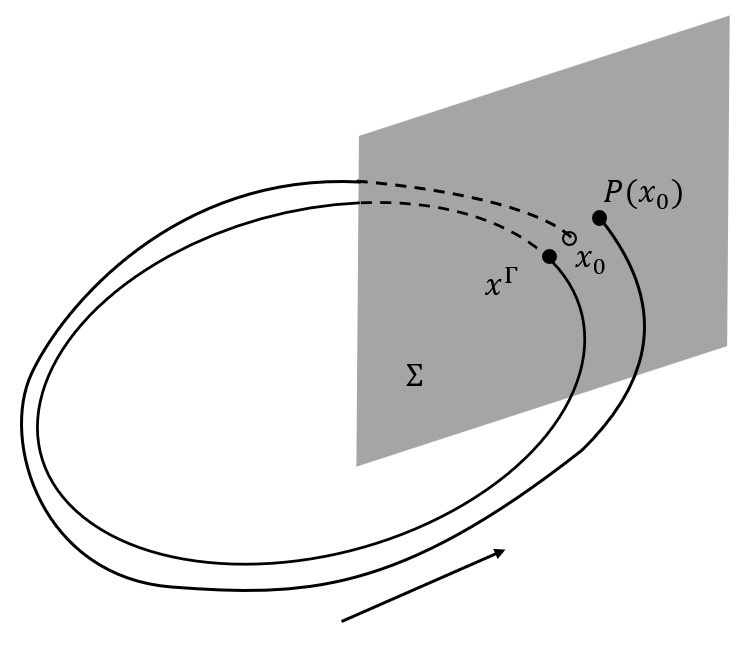
\includegraphics[width=0.5\textwidth]{figures/Map.jpg}
    \caption{Poincar\'e map.}
    \label{fig:map}
\end{figure}

Starting from an initial condition $x_{0}$ on the hyperplane $\Sigma$, after propagating the
trajectory returns to the hyperplane at $P(x_{0})$. If the trajectory is precisely periodic, the
trajectory will return to the same point, $x^{\Gamma}$. The Poincar\'e map then is the
2-dimensional representation of the hyperplane, displaying only the trajectory crossings. Note that
the axes of the map need not be position components but could also be velocity, energy, etc.
Similar mappings are used in this investigation to more efficiently analyze and compare manifold
trajectories of different orbits.
